% My Tool Box: introduction slides (Beamer, 16:9).
% Build with ./build.sh (pdflatex + latexmk); figures come from ../manual/figures.
\documentclass[10pt,aspectratio=169]{beamer}

\usetheme[progressbar=frametitle,numbering=fraction,block=fill,sectionpage=none]{metropolis}
\usepackage[T1]{fontenc}
\usepackage{lmodern}
\usepackage[scaled=0.95]{helvet}
\renewcommand{\familydefault}{\sfdefault}
% Latin Modern for mathematics (the T1 sans text font has no Greek capitals).
\usefonttheme[onlymath]{serif}
\usepackage{amsmath}
\usepackage{booktabs}
\usepackage{tabularx}
\usepackage{listings}
\usepackage[listings]{tcolorbox}
\usepackage{tikz}
\usetikzlibrary{positioning,shapes.misc,arrows.meta,calc,fit,backgrounds}
\usepackage{pgfplots}
\pgfplotsset{compat=1.18}
\graphicspath{{../manual/figures/}{figures/}}

% ---------------------------------------------------------------------------
% Palette (matches the environment dashboards)
% ---------------------------------------------------------------------------
\definecolor{ink}{HTML}{1F2430}
\definecolor{night}{HTML}{0E1117}
\definecolor{panel}{HTML}{151A23}
\definecolor{paper}{HTML}{F7F8FA}
\definecolor{rule}{HTML}{E3E6EB}
\definecolor{muted}{HTML}{6B7280}
\definecolor{accent}{HTML}{2563EB}
\definecolor{accentlight}{HTML}{4C9AFF}
\definecolor{green}{HTML}{059669}
\definecolor{orange}{HTML}{EA580C}
\definecolor{pink}{HTML}{DB2777}
\definecolor{purple}{HTML}{7C3AED}
\definecolor{cyan}{HTML}{0891B2}
\definecolor{amber}{HTML}{CA8A04}

\setbeamercolor{normal text}{fg=ink,bg=white}
\setbeamercolor{alerted text}{fg=orange}
\setbeamercolor{example text}{fg=green}
\setbeamercolor{frametitle}{fg=white,bg=panel}
\setbeamercolor{progress bar}{fg=accentlight,bg=rule}
\setbeamercolor{title separator}{fg=accentlight}
\setbeamercolor{block title}{fg=ink,bg=rule}
\setbeamercolor{block body}{fg=ink,bg=paper}
\setbeamerfont{frametitle}{size=\large,series=\bfseries}
\setbeamerfont{footnote}{size=\tiny}
\setbeamertemplate{frame footer}{\color{muted}My Tool Box 1.2}
\setbeamerfont{page number in head/foot}{size=\tiny}
\setbeamercolor{page number in head/foot}{fg=muted}

% ---------------------------------------------------------------------------
% Helpers
% ---------------------------------------------------------------------------
\newcommand{\code}[1]{\texttt{#1}}
\newcommand{\muted}[1]{{\color{muted}#1}}
% Big-number tile: \stat{colour}{number}{label}
\newcommand{\stat}[3]{%
  \begin{tikzpicture}
    \node[rounded corners=4pt,fill=#1!8,draw=#1!45,line width=0.6pt,
          minimum width=3.35cm,minimum height=2.05cm,inner sep=0pt] (b) {};
    \node[font=\bfseries\fontsize{24}{26}\selectfont,text=#1] at ($(b.center)+(0,0.28)$) {#2};
    \node[font=\scriptsize,text=ink,align=center,text width=3.1cm] at ($(b.center)+(0,-0.52)$) {#3};
  \end{tikzpicture}}
% Pill label
\newcommand{\pill}[2]{\tikz[baseline=(p.base)]\node[rounded corners=6pt,fill=#1!12,text=#1!70!black,
  font=\scriptsize\bfseries,inner xsep=5pt,inner ysep=2pt] (p) {#2};}

\lstdefinestyle{py}{
  language=Python,
  basicstyle=\ttfamily\fontsize{7.3}{8.9}\selectfont\color{ink},
  keywordstyle=\color{accent}\bfseries,
  stringstyle=\color{green},
  commentstyle=\color{muted}\itshape,
  showstringspaces=false,
  columns=fullflexible,
  keepspaces=true,
  backgroundcolor=\color{paper},
  frame=single,framerule=0pt,
  xleftmargin=4pt,xrightmargin=4pt,aboveskip=2pt,belowskip=2pt,
  morekeywords={as},
}
\lstdefinestyle{sh}{
  language={},
  basicstyle=\ttfamily\fontsize{7.3}{8.9}\selectfont\color{white},
  columns=fullflexible,keepspaces=true,
}
\lstset{style=py}
% Rounded code panels (one box per listing, no per-line seams).
\newtcblisting{pycode}{listing only,colback=paper,colframe=rule,boxrule=0.4pt,arc=3pt,
  left=5pt,right=5pt,top=3pt,bottom=3pt,
  listing options={style=py,backgroundcolor={},frame=none,xleftmargin=0pt,xrightmargin=0pt}}
\newtcblisting{shcode}{listing only,colback=panel,colframe=panel,boxrule=0pt,arc=3pt,
  left=5pt,right=5pt,top=3pt,bottom=3pt,
  listing options={style=sh,backgroundcolor={},frame=none,xleftmargin=0pt,xrightmargin=0pt}}

\tikzset{
  box/.style={rounded corners=3pt,draw=#1!55,fill=#1!7,line width=0.6pt,
              font=\scriptsize,align=center,inner sep=3pt},
  box/.default=accent,
  layer/.style={rounded corners=5pt,draw=rule,fill=paper,line width=0.6pt},
  arrow/.style={-{Stealth[length=2.2mm]},line width=0.7pt,color=muted},
}

% ---------------------------------------------------------------------------
% Numbers (measured with benchmarks/benchmark_envs.py and benchmark_vector.py)
% ---------------------------------------------------------------------------
% Figures quoted on the slides. Regenerate after running the benchmarks.
\newcommand{\NumFamilies}{8}
\newcommand{\NumIds}{18}
\newcommand{\NumContinuous}{6}
\newcommand{\NumThroughput}{TBD}
\newcommand{\NumTests}{TBD}
\newcommand{\NumHandbookPages}{TBD}
\newcommand{\NumEvalEpisodes}{TBD}
\newcommand{\FigTitleA}{power_grid.png}
\newcommand{\FigTitleB}{platoon.png}
\newcommand{\FigPowerGrid}{power_grid.png}
\newcommand{\FigPlatoon}{platoon.png}
\newcommand{\ThroughputTitle}{PowerGrid-v0, 16 buses (placeholder)}
\newcommand{\ThroughputNative}{(1,1e4) (16,1.5e5) (64,5e5) (256,1.5e6) (1024,3e6)}
\newcommand{\ThroughputSync}{(1,1e4) (16,1.1e4) (64,1.1e4) (256,1.1e4)}
\newcommand{\PerfRows}{Kuramoto, 50 oscillators & 2.36 ms & TBD\\ AJLATT, 4 robots & 90 ms & TBD\\}
\newcommand{\BaselineRows}{PowerGrid & droop control $u_i = -k\,\omega_i$ & TBD & TBD\\}


\title{My Tool Box}
\subtitle{Networked multi-agent control environments, classical MARL algorithms and research utilities for Python}
\author{Dongming Wang}
\date{Version 1.2}

\begin{document}

% ---------------------------------------------------------------------------
\begin{frame}[plain]
  \begin{tikzpicture}[remember picture,overlay]
    \fill[night] (current page.south west) rectangle (current page.north east);
    \fill[accentlight] ($(current page.north west)+(0,-0.1)$) rectangle (current page.north east);
    \node[anchor=north west,inner sep=0pt] at ($(current page.north west)+(0.95,-1.25)$) {%
      \begin{minipage}{7.3cm}\raggedright
        {\color{white}\fontsize{32}{36}\selectfont\bfseries My Tool Box}\\[10pt]
        {\color{accentlight}\fontsize{14}{18}\selectfont Networked multi-agent control\\
         environments, classical MARL\\ algorithms and research tools}\\[18pt]
        {\color{white!75!night}\small Gymnasium API\enspace$\cdot$\enspace continuous states and actions\\
         native batched simulation\enspace$\cdot$\enspace reference controllers\\
         MAPPO, MADDPG, QMIX and more, trained on the environments}\\[24pt]
        {\color{white}\small Dongming Wang}\\[3pt]
        {\color{white!55!night}\scriptsize Version 1.2\enspace$\cdot$\enspace github.com/EricDMW/My\_Tool\_Box}
      \end{minipage}};
    \node[anchor=north east,inner sep=0pt] (a) at ($(current page.north east)+(-0.6,-0.72)$)
      {\includegraphics[width=6.4cm]{\FigTitleA}};
    \node[anchor=north,inner sep=0pt] (b) at ($(a.south)+(0,-0.2)$)
      {\includegraphics[width=6.4cm]{\FigTitleB}};
    \draw[white!25!night,line width=0.8pt] (a.south west) rectangle (a.north east);
    \draw[white!25!night,line width=0.8pt] (b.south west) rectangle (b.north east);
  \end{tikzpicture}
\end{frame}

% ---------------------------------------------------------------------------
\begin{frame}{At a glance}
  \centering
  \stat{accent}{\NumFamilies}{environment families\\(\NumIds{} registered ids)}\hfill
  \stat{green}{\NumAlgorithms}{classical MARL algorithms\\trained on the environments}\hfill
  \stat{orange}{\NumThroughput}{agent-steps per second\\(256 copies, one CPU core)}\hfill
  \stat{purple}{\NumTests}{tests, CI on\\Python 3.9 to 3.12}

  \vspace{14pt}
  \begin{columns}[T,onlytextwidth]
    \column{0.32\textwidth}
    \textbf{\color{accent}env\_lib}\quad simulation\\[2pt]
    \footnotesize Oscillator networks, consensus and formation, power-grid frequency control,
    vehicle platoons, multi-robot target tracking, cooperative physics and
    communication benchmarks, behind one Gymnasium interface; \NumContinuous{} families with
    continuous states and actions.
    \column{0.32\textwidth}
    \textbf{\color{accent}marl\_algorithms}\quad learning\\[2pt]
    \footnotesize IPPO, MAPPO, MADDPG, MATD3, IQL, VDN and QMIX on one small core, trained
    on batched copies of the environments and evaluated against their classical
    controllers.
    \column{0.32\textwidth}
    \textbf{\color{accent}toolkit}\quad research workflow\\[2pt]
    \footnotesize Publication-quality plots with confidence bands, PyTorch policy and value
    networks, and reproducible experiment parameters, in the same install.
  \end{columns}
\end{frame}

% ---------------------------------------------------------------------------
\begin{frame}{Built for networked multi-agent control}
  \centering
  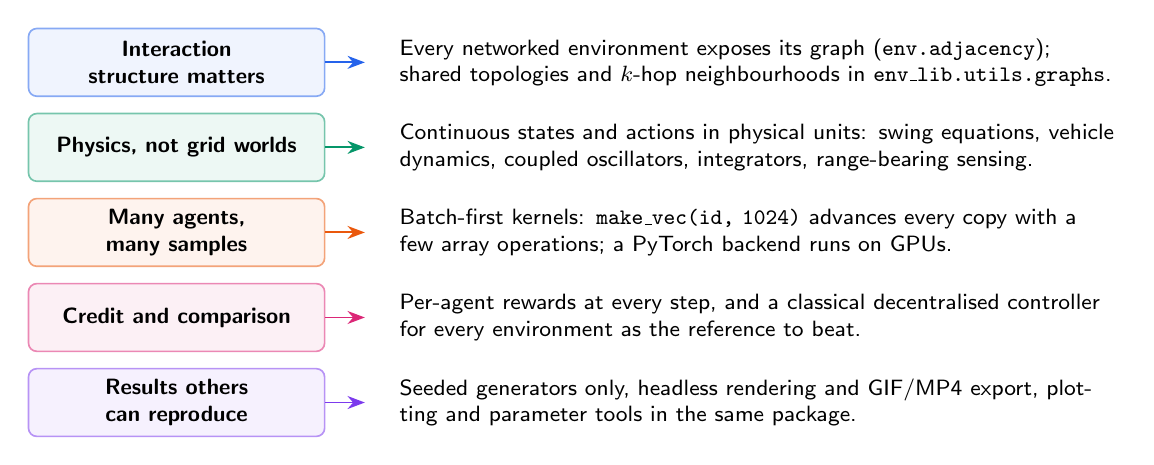
\begin{tikzpicture}
    \foreach \i/\need/\feat/\col in {
      0/{Interaction structure matters}/{Every networked environment exposes its graph (\code{env.adjacency}); shared
        topologies and $k$-hop neighbourhoods in \code{env\_lib.utils.graphs}.}/accent,
      1/{Physics, not grid worlds}/{Continuous states and actions in physical units: swing equations, vehicle
        dynamics, coupled oscillators, integrators, range-bearing sensing.}/green,
      2/{Many agents, many samples}/{Batch-first kernels: \code{make\_vec(id, 1024)} advances every copy with a
        few array operations; a PyTorch backend runs on GPUs.}/orange,
      3/{Credit and comparison}/{Per-agent rewards at every step, and a classical decentralised controller for
        every environment as the reference to beat.}/pink,
      4/{Results others can reproduce}/{Seeded generators only, headless rendering and GIF/MP4 export, plotting
        and parameter tools in the same package.}/purple%
    }{
      \node[box=\col,minimum height=0.86cm,text width=3.55cm,font=\footnotesize\bfseries,anchor=west,
            execute at begin node={\hyphenpenalty=10000}]
        (n\i) at (0,-\i*1.08) {\need};
      \node[anchor=west,text width=9.1cm,font=\footnotesize,align=left] (f\i) at (4.6,-\i*1.08) {\feat};
      \draw[arrow,color=\col] (n\i.east) -- ++(0.5,0);
    }
  \end{tikzpicture}
\end{frame}

% ---------------------------------------------------------------------------
\begin{frame}{Design}
  \centering
  \resizebox{\textwidth}{!}{%
  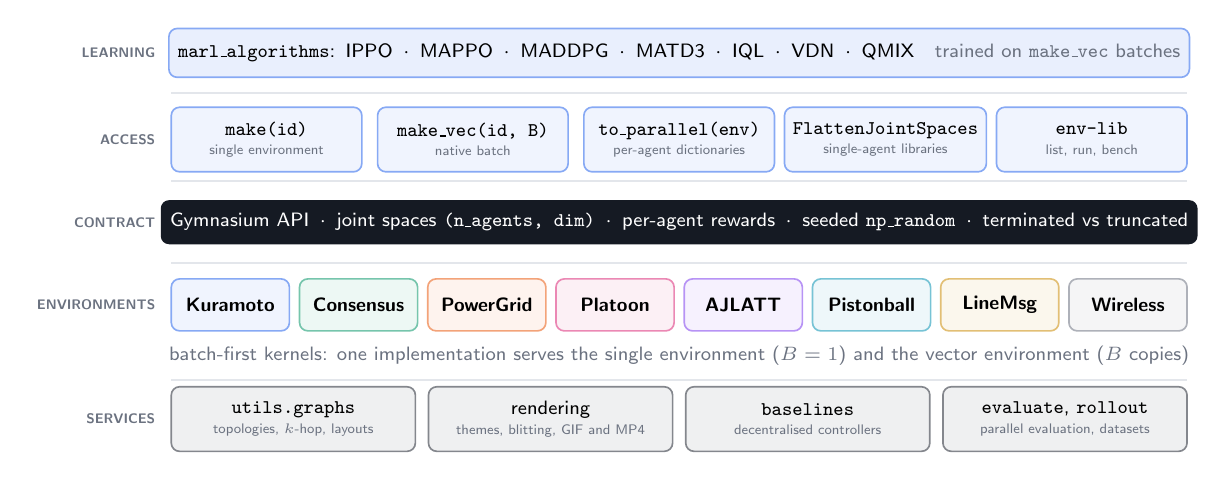
\begin{tikzpicture}[x=1cm,y=1cm]
    % Learning layer
    \node[fill=accent!10,draw=accent!55,rounded corners=3pt,line width=0.6pt,minimum width=12.9cm,
          minimum height=0.62cm,font=\scriptsize] at (7.15,4.35)
      {\code{marl\_algorithms}:\enspace IPPO\enspace$\cdot$\enspace MAPPO\enspace$\cdot$\enspace
       MADDPG\enspace$\cdot$\enspace MATD3\enspace$\cdot$\enspace IQL\enspace$\cdot$\enspace
       VDN\enspace$\cdot$\enspace QMIX\quad{\color{muted}trained on \code{make\_vec} batches}};
    \draw[rule,line width=0.6pt] (0.7,3.84) -- (13.6,3.84);
    % Access layer
    \foreach \lab/\sub [count=\k from 0] in {\code{make(id)}/single environment,
        \code{make\_vec(id{,} B)}/native batch,\code{to\_parallel(env)}/per-agent dictionaries,
        \code{FlattenJointSpaces}/single-agent libraries,\code{env-lib}/{list{,} run{,} bench}}{
      \node[box=accent,minimum width=2.42cm,minimum height=0.82cm] (a\k) at (1.91+\k*2.62,3.25)
        {\lab\\[-1pt]{\tiny\color{muted}\sub}};
    }
    % Contract
    \node[fill=panel,rounded corners=3pt,minimum width=12.9cm,minimum height=0.56cm,text=white,
          font=\scriptsize] (api) at (7.15,2.2)
      {Gymnasium API\enspace$\cdot$\enspace joint spaces \code{(n\_agents, dim)}\enspace$\cdot$\enspace
       per-agent rewards\enspace$\cdot$\enspace seeded \code{np\_random}\enspace$\cdot$\enspace
       terminated vs truncated};
    % Environments
    \foreach \name/\col [count=\k from 0] in {Kuramoto/accent,Consensus/green,PowerGrid/orange,
        Platoon/pink,AJLATT/purple,Pistonball/cyan,LineMsg/amber,Wireless/muted}{
      \node[box=\col,minimum width=1.5cm,minimum height=0.66cm,font=\scriptsize\bfseries]
        (e\k) at (1.45+\k*1.6286,1.15) {\name};
    }
    \node[font=\scriptsize,text=muted] at (7.15,0.5)
      {batch-first kernels: one implementation serves the single environment ($B = 1$) and the vector environment ($B$ copies)};
    % Services
    \node[box=ink,minimum width=3.1cm,minimum height=0.82cm] at (2.25,-0.3)
      {\code{utils.graphs}\\[-1pt]{\tiny\color{muted}topologies, $k$-hop, layouts}};
    \node[box=ink,minimum width=3.1cm,minimum height=0.82cm] at (5.5167,-0.3)
      {rendering\\[-1pt]{\tiny\color{muted}themes, blitting, GIF and MP4}};
    \node[box=ink,minimum width=3.1cm,minimum height=0.82cm] at (8.7833,-0.3)
      {\code{baselines}\\[-1pt]{\tiny\color{muted}decentralised controllers}};
    \node[box=ink,minimum width=3.1cm,minimum height=0.82cm] at (12.05,-0.3)
      {\code{evaluate}, \code{rollout}\\[-1pt]{\tiny\color{muted}parallel evaluation, datasets}};
    % Layer labels
    \foreach \y/\lab in {4.35/learning,3.25/access,2.2/contract,1.15/environments,-0.3/services}{
      \node[font=\tiny\bfseries,text=muted,anchor=east] at (0.62,\y) {\MakeUppercase{\lab}};
    }
    \draw[rule,line width=0.6pt] (0.7,2.72) -- (13.6,2.72);
    \draw[rule,line width=0.6pt] (0.7,1.68) -- (13.6,1.68);
    \draw[rule,line width=0.6pt] (0.7,0.2) -- (13.6,0.2);
  \end{tikzpicture}}
\end{frame}

% ---------------------------------------------------------------------------
\begin{frame}{Environment suite}
  \centering
  \setlength{\tabcolsep}{2pt}
  \begin{tabular}{ccc}
    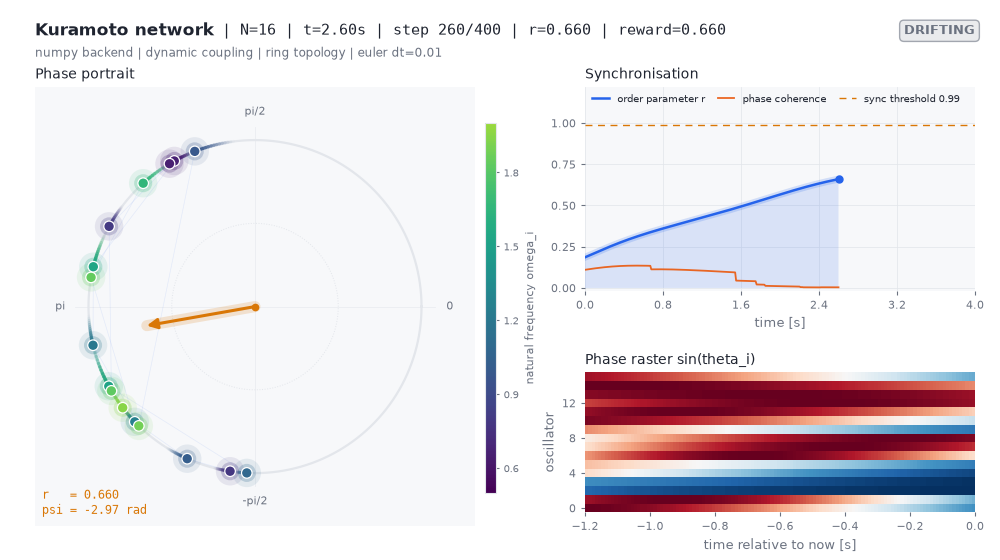
\includegraphics[width=0.322\textwidth]{kuramoto.png} &
    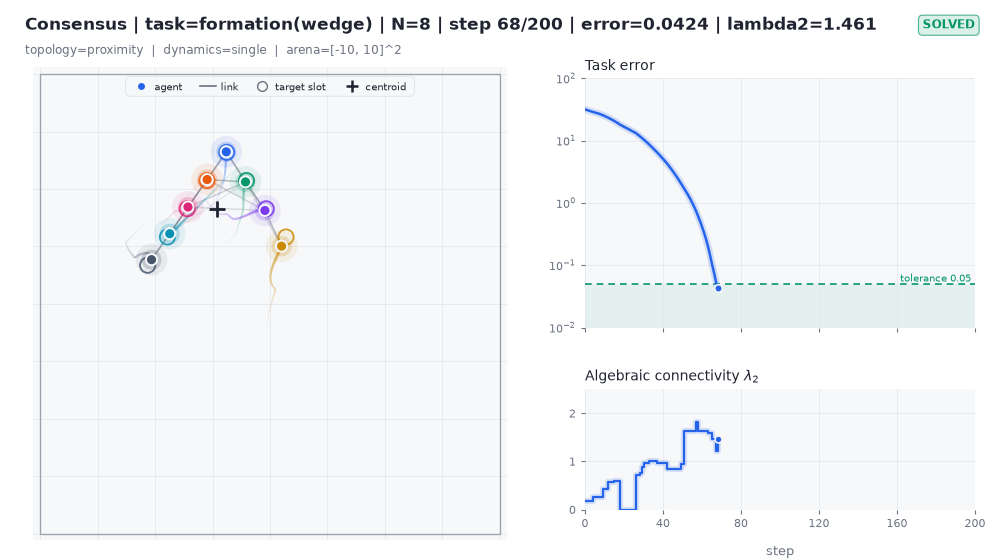
\includegraphics[width=0.322\textwidth]{formation.png} &
    \includegraphics[width=0.322\textwidth]{\FigPowerGrid} \\[-1pt]
    \scriptsize Kuramoto synchronisation & \scriptsize Formation control & \scriptsize Power-grid frequency control \\[4pt]
    \includegraphics[width=0.322\textwidth]{\FigPlatoon} &
    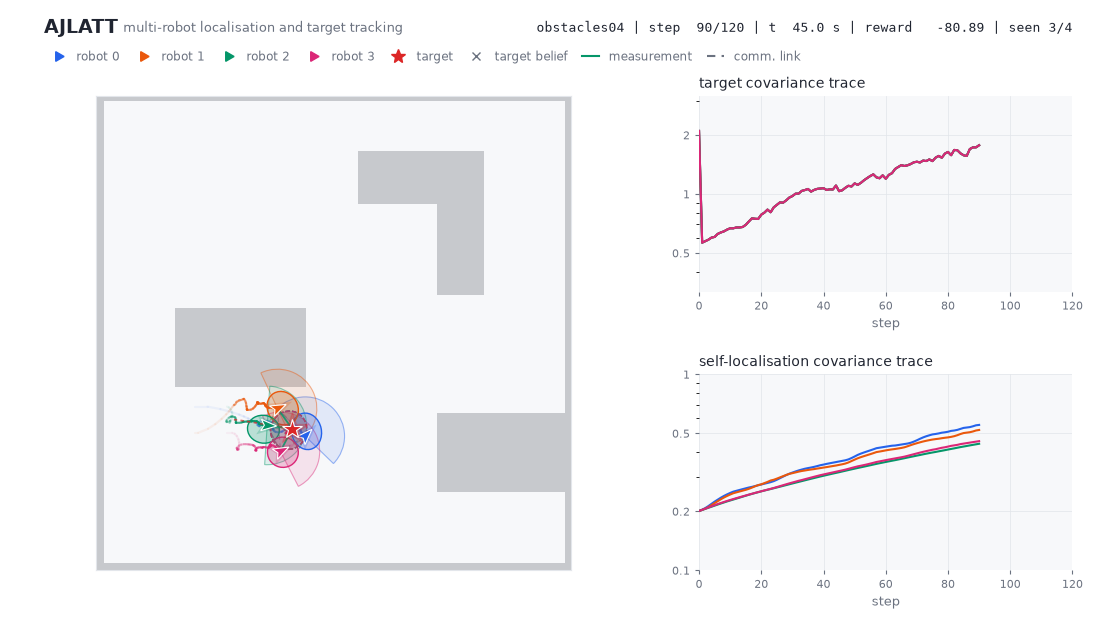
\includegraphics[width=0.322\textwidth]{ajlatt.png} &
    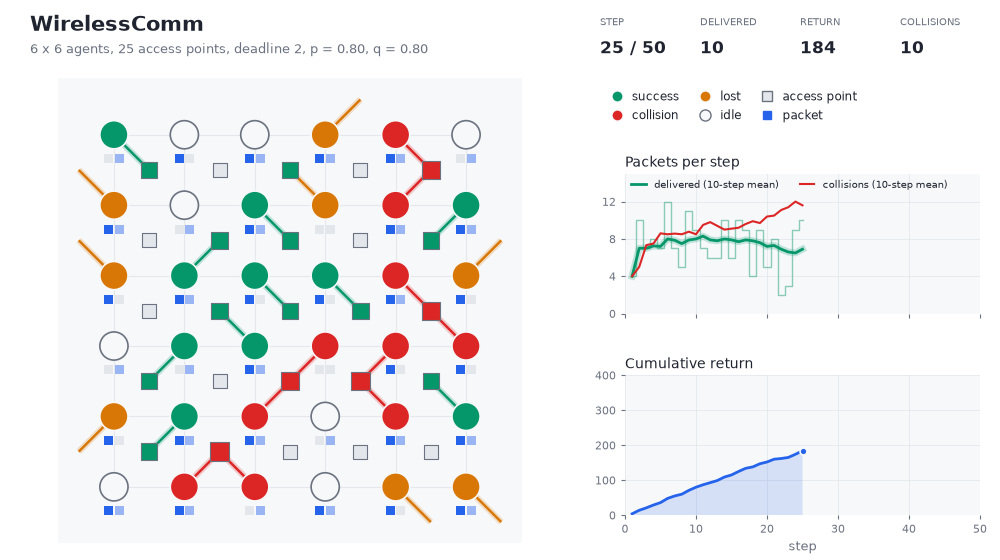
\includegraphics[width=0.322\textwidth]{wireless.png} \\[-1pt]
    \scriptsize Vehicle platoon (CACC) & \scriptsize Multi-robot target tracking & \scriptsize Wireless access grid
  \end{tabular}
\end{frame}

% ---------------------------------------------------------------------------
\begin{frame}{Continuous states and actions}
  \scriptsize
  \renewcommand{\arraystretch}{1.35}
  \begin{tabularx}{\textwidth}{@{}l>{\raggedright\arraybackslash}X>{\raggedright\arraybackslash}p{3.7cm}l@{}}
    \toprule
    \textbf{Environment} & \textbf{State and dynamics} & \textbf{Action per agent} & \textbf{Interaction graph}\\
    \midrule
    \color{orange}\textbf{PowerGrid} & bus phase angles and frequencies; swing equations & bounded power injection & transmission network\\
    \color{pink}\textbf{Platoon} & gaps, speeds and accelerations; actuator lag & commanded acceleration & V2V topology\\
    \color{green}\textbf{Consensus, Formation} & planar positions (and velocities); single or double integrator & velocity or acceleration & fixed or proximity graph\\
    \color{accent}\textbf{Kuramoto} & oscillator phases; phase-coupled dynamics & control input and coupling gains & coupling network\\
    \color{purple}\textbf{AJLATT} & robot and target poses, EKF beliefs & linear and angular velocity & communication range\\
    \color{cyan}\textbf{Pistonball} & rigid-body physics (pymunk) & piston velocity (or discrete) & line of pistons\\
    \bottomrule
  \end{tabularx}

  \vspace{10pt}
  \footnotesize
  \muted{Observations are stacked per agent, \code{(n\_agents, obs\_dim)} \code{float32}, in physical units
  with documented layouts (\code{env.observation\_layout}). LineMsg and WirelessComm add discrete
  networked benchmarks.}
\end{frame}

% ---------------------------------------------------------------------------
\begin{frame}[fragile]{One interface, from a single run to large batches}
  \begin{columns}[T,onlytextwidth]
    \column{0.57\textwidth}
    \footnotesize\textbf{Python}\\[2pt]
\begin{pycode}
import env_lib

env = env_lib.make("PowerGrid-v0")
obs, info = env.reset(seed=0)    # (agents, obs_dim)
policy = env_lib.baseline_policy(env)
obs, r, term, trunc, info = env.step(policy(obs))
info["agent_rewards"]            # (agents,)

envs = env_lib.make_vec("PowerGrid-v0", num_envs=1024)
obs, _ = envs.reset(seed=0)      # (1024, agents, dim)
print(env_lib.evaluate(envs, policy, n_episodes=1024))
\end{pycode}
    \column{0.39\textwidth}
    \footnotesize\textbf{Existing learners}\\[2pt]
\begin{pycode}
from env_lib.wrappers import (
  FlattenJointSpaces, to_parallel)
sb3_env = FlattenJointSpaces(env)
pettingzoo_env = to_parallel(env)
\end{pycode}
    \vspace{6pt}
    \textbf{Shell}\\[2pt]
\begin{shcode}
$ env-lib list --continuous
$ env-lib describe Platoon-v0
$ env-lib run Platoon-v0 --gif f.gif
$ env-lib evaluate PowerGrid-v0
$ env-lib bench Platoon-v0
\end{shcode}
  \end{columns}
\end{frame}

% ---------------------------------------------------------------------------
\begin{frame}{Batch-first simulation}
  \begin{columns}[c,onlytextwidth]
    \column{0.4\textwidth}
    \small
    Each continuous environment is written once, for arrays with a leading batch axis:
    \[
      x_{t+1} = f(x_t, u_t),\quad x_t \in \mathbb{R}^{B \times n \times d}.
    \]
    \vspace{-4pt}
    \begin{itemize}\setlength\itemsep{2pt}\footnotesize
      \item single environment: $B = 1$;
      \item vector environment: $B$ copies, same array operations;
      \item Gymnasium autoreset modes;
      \item copy 0 reproduces the single environment.
    \end{itemize}
    \column{0.57\textwidth}
    \centering
    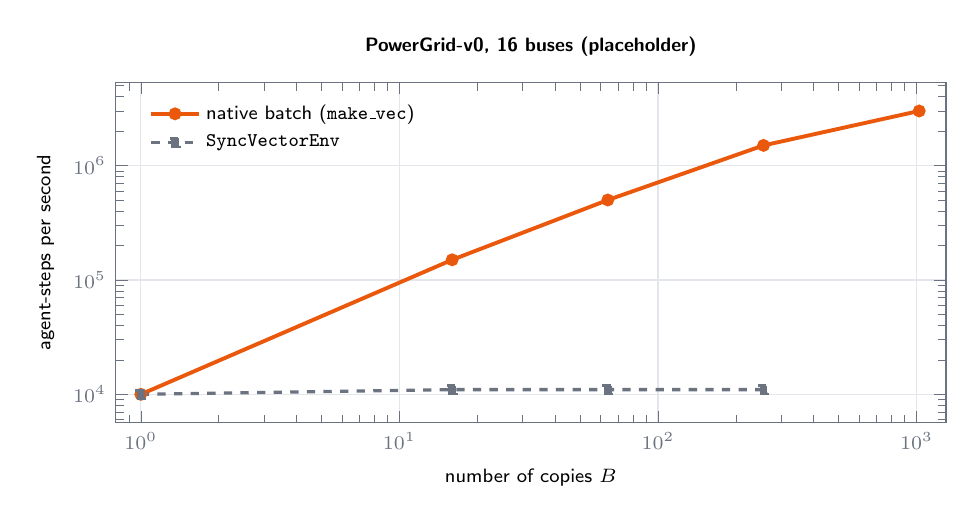
\begin{tikzpicture}
      \begin{loglogaxis}[
        width=\linewidth,height=5.9cm,
        xlabel={number of copies $B$},ylabel={agent-steps per second},
        xmin=0.8,xmax=1300,
        grid=major,grid style={rule},
        axis line style={muted},tick style={muted},
        tick label style={font=\scriptsize,text=muted},label style={font=\scriptsize},
        legend style={font=\scriptsize,draw=none,fill=none,at={(0.03,0.97)},anchor=north west},
        legend cell align=left,
        title style={font=\scriptsize\bfseries},title={\ThroughputTitle},
      ]
        \addplot[color=orange,line width=1.4pt,mark=*,mark size=1.6pt] coordinates {\ThroughputNative};
        \addlegendentry{native batch (\code{make\_vec})}
        \addplot[color=muted,line width=1.2pt,mark=square*,mark size=1.4pt,dashed] coordinates {\ThroughputSync};
        \addlegendentry{\code{SyncVectorEnv}}
      \end{loglogaxis}
    \end{tikzpicture}
  \end{columns}
\end{frame}

% ---------------------------------------------------------------------------
\begin{frame}{Performance}
  \begin{columns}[T,onlytextwidth]
    \column{0.52\textwidth}
    \footnotesize
    \textbf{Single environment, time per step}\\[3pt]
    \renewcommand{\arraystretch}{1.12}
    \begin{tabularx}{\linewidth}{@{}X r r@{}}
      \toprule
      Environment & before 1.0 & 1.2\\
      \midrule
      \PerfRows
      \bottomrule
    \end{tabularx}
    \column{0.44\textwidth}
    \footnotesize
    \textbf{Where the speed comes from}\\[3pt]
    \begin{itemize}\setlength\itemsep{2pt}
      \item vectorised dynamics, no Python loops over agents;
      \item exact batched ray casting on occupancy grids;
      \item covariance intersection by projected Newton with analytic derivatives;
      \item persistent artists and blitting for rendering;
      \item optional dependencies imported only when used.
    \end{itemize}
    \vspace{4pt}
    \muted{Seeded trajectories were checked against the previous implementation
    wherever the refactor was not meant to change results.}
  \end{columns}
\end{frame}

% ---------------------------------------------------------------------------
\begin{frame}{A reference controller for every environment}
  \footnotesize
  \renewcommand{\arraystretch}{1.25}
  \begin{tabularx}{\textwidth}{@{}l>{\raggedright\arraybackslash}Xrr@{}}
    \toprule
    \textbf{Environment} & \textbf{Decentralised baseline} & \textbf{Random} & \textbf{Baseline}\\
    \midrule
    \BaselineRows
    \bottomrule
  \end{tabularx}

  \vspace{8pt}
  \muted{Mean return over \NumEvalEpisodes{} seeded episodes (8 for AJLATT, 16 for Pistonball; higher is better).
  \code{env\_lib.baseline\_policy(env)} returns the controller as a function of the observation,
  so the same call drives one environment or a batch of thousands.}
\end{frame}

% ---------------------------------------------------------------------------
\begin{frame}[fragile]{Classical MARL algorithms, trained on the environments}
  \begin{columns}[T,onlytextwidth]
    \column{0.40\textwidth}
    \footnotesize
    \renewcommand{\arraystretch}{1.15}
    \begin{tabularx}{\linewidth}{@{}l>{\raggedright\arraybackslash}X@{}}
      \toprule
      Algorithm & Family, actions\\
      \midrule
      IPPO, MAPPO & on-policy; continuous or discrete\\
      MADDPG, MATD3 & off-policy actor-critic; continuous\\
      IQL, VDN, QMIX & value-based; discrete\\
      \bottomrule
    \end{tabularx}

    \vspace{8pt}
    One core serves all seven: per-agent view of the joint spaces, batched
    experience collection, buffers, shared or per-agent networks, two
    training loops.
    \vspace{6pt}
\begin{shcode}
$ marl-train run mappo PowerGrid-v0
$ marl-train compare PowerGrid-v0 \
    --seeds 0 1 2      # baselines
\end{shcode}
    \column{0.57\textwidth}
    \footnotesize
    \textbf{Tuned presets, one CPU core, 64 seeded episodes}\\[3pt]
    \renewcommand{\arraystretch}{1.15}
    \setlength{\tabcolsep}{4.5pt}
    \begin{tabular}{@{}llrrrr@{}}
      \toprule
      Algorithm & Environment & Time & Random & Trained & Baseline\\
      \midrule
      \MarlRows
      \bottomrule
    \end{tabular}\\[4pt]
    \muted{Mean return, higher is better; the baseline is the environment's
    classical controller.}
  \end{columns}
\end{frame}

% ---------------------------------------------------------------------------
\begin{frame}{Research utilities in the same install}
  \begin{columns}[c,onlytextwidth]
    \column{0.56\textwidth}
    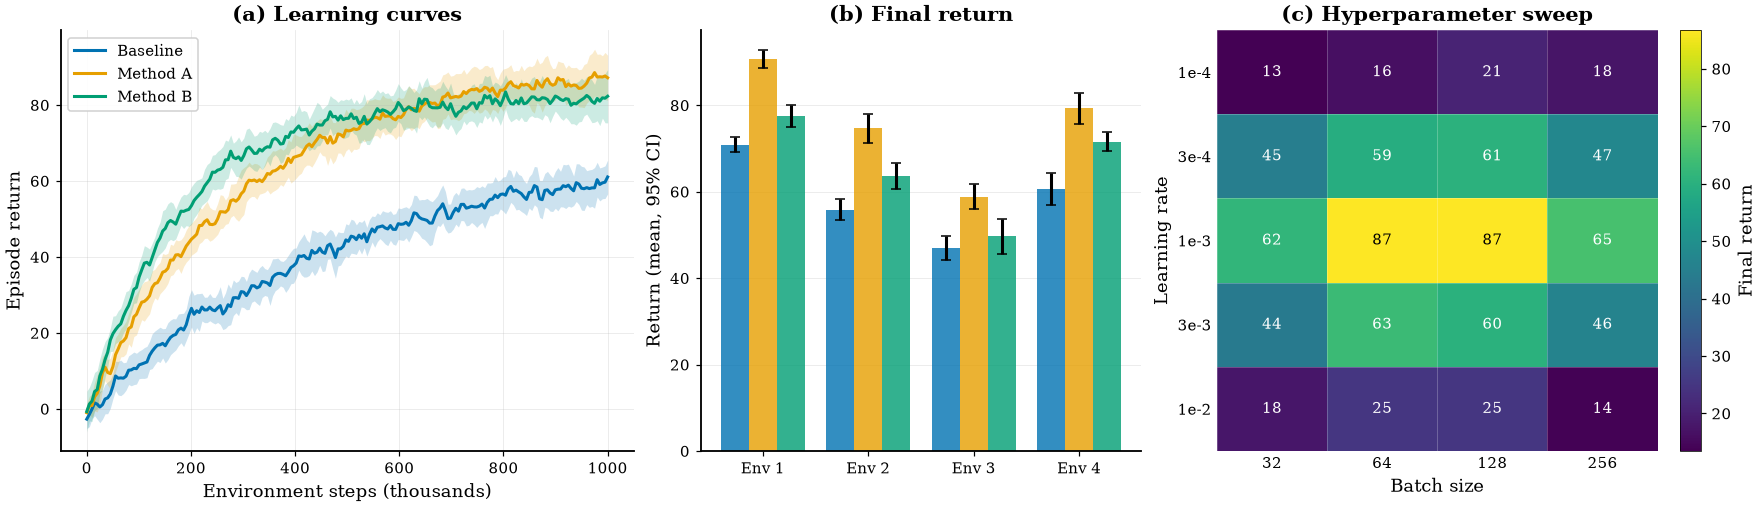
\includegraphics[width=\linewidth]{plotkit_gallery.png}
    \column{0.41\textwidth}
    \footnotesize
    \textbf{\color{accent}plotkit}\enspace learning curves with confidence bands, grouped bars,
    heatmaps, colour-blind-safe palette, vector export.\\[7pt]
    \textbf{\color{accent}neural\_toolkit}\enspace MLP, CNN, RNN and Transformer policies, value and
    Q-networks, encoders and decoders (PyTorch).\\[7pt]
    \textbf{\color{accent}parakit}\enspace save, load and validate \code{argparse} experiment
    parameters; optional editor.\\[7pt]
    \textbf{\color{accent}recording}\enspace \code{record\_episode(env, policy, "run.gif")} for every
    environment, in dark and light themes.
  \end{columns}
\end{frame}

% ---------------------------------------------------------------------------
\begin{frame}{Engineering quality}
  \centering
  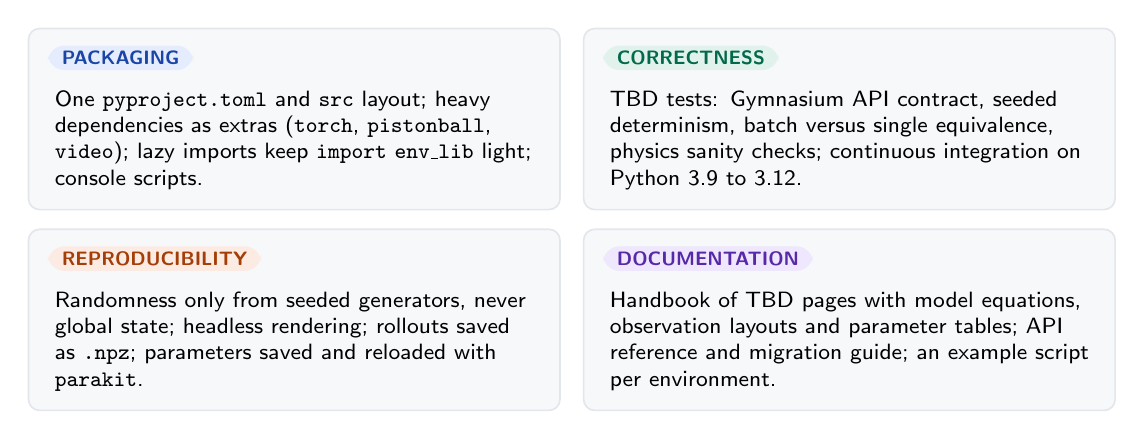
\begin{tikzpicture}
    \foreach \x/\y/\col/\tag/\body in {
      0/0/accent/PACKAGING/{One \code{pyproject.toml} and \code{src} layout; heavy dependencies as extras
        (\code{torch}, \code{pistonball}, \code{video}); lazy imports keep \code{import env\_lib} light;
        console scripts.},
      7.05/0/green/CORRECTNESS/{\NumTests{} tests: Gymnasium API contract, seeded determinism, batch versus single
        equivalence, physics sanity checks; continuous integration on Python 3.9 to 3.12.},
      0/-2.55/orange/REPRODUCIBILITY/{Randomness only from seeded generators, never global state; headless
        rendering; rollouts saved as \code{.npz}; parameters saved and reloaded with \code{parakit}.},
      7.05/-2.55/purple/DOCUMENTATION/{Handbook of \NumHandbookPages{} pages with model equations, observation
        layouts and parameter tables; API reference and migration guide; an example script per environment.}%
    }{
      \node[anchor=north west,rounded corners=4pt,fill=paper,draw=rule,line width=0.6pt,
            minimum width=6.75cm,minimum height=2.3cm] (c) at (\x,\y) {};
      \node[anchor=north west,rounded corners=6pt,fill=\col!12,text=\col!70!black,font=\scriptsize\bfseries,
            inner xsep=5pt,inner ysep=2pt] at ($(c.north west)+(0.25,-0.22)$) {\tag};
      \node[anchor=north west,text width=6.2cm,font=\footnotesize,align=left]
        at ($(c.north west)+(0.22,-0.68)$) {\body};
    }
  \end{tikzpicture}
\end{frame}

% ---------------------------------------------------------------------------
\begin{frame}[fragile]{Get started}
  \begin{columns}[c,onlytextwidth]
    \column{0.55\textwidth}
\begin{shcode}
$ git clone https://github.com/EricDMW/My_Tool_Box
$ cd My_Tool_Box && pip install -e ".[all]"
$ env-lib list
$ env-lib run Platoon-v0 --gif platoon.gif
\end{shcode}
    \vspace{8pt}
    \small
    \begin{tabular}{@{}ll@{}}
      Slides & \code{docs/slides/my\_tool\_box\_slides.pdf}\\
      Handbook & \code{docs/manual/main.pdf}\\
      Examples & \code{examples/} (one script per environment)\\
      Changes & \code{CHANGELOG.md}\\
    \end{tabular}
    \column{0.42\textwidth}
    \centering
    \includegraphics[width=\linewidth]{\FigPlatoon}
  \end{columns}
\end{frame}

\end{document}
